%% This document created by Scientific Word (R) Version 3.0

\documentclass[12pt,a4paper]{article}

\textwidth 15cm \textheight 21cm  %A4: 210x297mm; letter: 216x279mm
\hoffset -0.5cm \topmargin -0.cm
%\oddsidemargin 0.0in \evensidemargin 0pt 
% \marginparwidth 0pt \marginparsep 0pt 

\usepackage{epsfig,subfigure,epstopdf}
\usepackage{multirow}
\usepackage{rotating}
\usepackage{graphicx}
\usepackage{amsmath}
\usepackage{amsfonts}
\usepackage{amssymb}
\usepackage{algorithm}
\usepackage{algorithmic}
%\usepackage{cleveref}
 \usepackage{refcheck}

%\usepackage{color}
\usepackage[usenames, dvipsnames]{color}
\newcommand{\tk}{\textcolor{Black}}
\newcommand{\tb}{\textcolor{blue}}
\newcommand{\tr}{\textcolor{red}}
\newcommand{\tg}{\textcolor{Green}}
\newcommand{\tc}{\textcolor{Cerulean}}
% ===
\newtheorem{theorem}{Theorem}
\newtheorem{acknowledgement}[theorem]{Acknowledgement}
\newtheorem{algorithm_01}[theorem]{Algorithm}
\newtheorem{axiom}[theorem]{Axiom}
\newtheorem{case}[theorem]{Case}
\newtheorem{claim}[theorem]{Claim}
\newtheorem{conclusion}[theorem]{Conclusion}
\newtheorem{condition}[theorem]{Condition}
\newtheorem{conjecture}[theorem]{Conjecture}
\newtheorem{corollary}[theorem]{Corollary}
\newtheorem{criterion}[theorem]{Criterion}
\newtheorem{definition}[theorem]{Definition}
\newtheorem{example}[theorem]{Example}
\newtheorem{exercise}[theorem]{Exercise}
\newtheorem{lemma}[theorem]{Lemma}
\newtheorem{notation}[theorem]{Notation}
\newtheorem{problem}[theorem]{Problem}
\newtheorem{proposition}[theorem]{Proposition}
\newtheorem{remark}[theorem]{Remark}
\newtheorem{solution}[theorem]{Solution}
\newtheorem{summary}[theorem]{Summary}
\newenvironment{proof}[1][Proof]{\textbf{#1.} }{\ \rule{0.5em}{0.5em}}

\begin{document}


\title{Put title here}
\author{[For internal reference only.]}
\date{\today}
\maketitle


\abstract{Put abstract here.\\
{\bf Keywords.} }

% ====================================================================

\setcounter{section}{-1}
\section{Outline}

% ====================================================================
\section{Introduction}
% ====================================================================

Main idea:
\cite{xyz}

Sections~\ref{sec:alg_01} and \ref{sec:alg_02} describe algoirhtm
environments.  Section~\ref{sec:tab} describes tables.
Section~\ref{sec:fig} describes figures.

% ====================================================================
\section{LaTeX Examples}
% ====================================================================


% ====================================================================
\subsection{Algorithm Type 1}
\label{sec:alg_01}
% ====================================================================

See Algorithm~\ref{alg:01} for an example. Reference:
\begin{itemize}
\item {\tt http://en.wikibooks.org/wiki/LaTeX/Algorithms\_and\_Pseudocode}
\item {\tt http://developer.berlios.de/docman/display\_doc.php?docid=800\&group\_id=3442}
\end{itemize}


\begin{algorithm}
\caption{Calculate $y = x^n$}
\label{alg1}
\begin{algorithmic}[1]
\REQUIRE $n \geq 0 \vee x \neq 0$
\ENSURE $y = x^n$
\STATE $y \Leftarrow 1$
\IF{$n < 0$}
\STATE $X \Leftarrow 1 / x$
\STATE $N \Leftarrow -n$
\ELSE
\STATE $X \Leftarrow x$
\STATE $N \Leftarrow n$
\ENDIF
\WHILE{$N \neq 0$}
\IF{$N$ is even}
\STATE $X \Leftarrow X \times X$
\STATE $N \Leftarrow N / 2$
\ELSE[$N$ is odd]
\STATE $y \Leftarrow y \times X$
\STATE $N \Leftarrow N - 1$
\ENDIF
\ENDWHILE
\end{algorithmic}
\label{alg:01}
\end{algorithm}


% ====================================================================
\subsection{Algorithm Type 2}
\label{sec:alg_02}
% ====================================================================

\begin{algorithm_01}
\label{alg:surrogate} \textbf{Surrogate-Assisted Search (SAS)}\\
\begin{tabular}{|lllll|}
\hline
%& & & & \\
%\item[(1)] Generate grid over the experimental region.
(1) & \multicolumn{3}{l}{Initialization: Choose initial experiment points and evaluate} & \\
    & \multicolumn{3}{l}{the corresponding function values.} & \\
%\item[(3)] Generate basis functions.
(2) & \multicolumn{3}{l}{Repeat until the effective points are found.} & \\

& (2.1) & \multicolumn{2}{l}{Update the surrogate surface.} & \\
& (2.2) & \multicolumn{2}{l}{Determine next possible experiment points} & \\
& (2.3) & \multicolumn{2}{l}{Perform function evaluations.} & \\
%& & & & \\
\hline
\end{tabular}
\end{algorithm_01}

% ====================================================================
\subsection{Table}
\label{sec:tab}
% ====================================================================
% --- table
%
% NOTE: ADD \usepackage{multirow} in the beginning
%
\begin{table}[thf]
  \centering
  \begin{tabular}{llllll}
    \hline
   & \multicolumn{3}{c}{PSO}                 &             \\ \cline{2-4}
   & Function & $x_{i}$ domain  & Optimum    & Reference    \\ \hline
\multirow{3}{*}{Type 1} & $f_{1}$  & $[3,13]$        & $1.21598D$ & \cite{KNG:96} \\
   & $f_{2}$ & & &  \\
   & $f_{3}$ & & &  \\ \hline
\multirow{3}{*}{Type 2} & $f_{4}$  &   & & \\
   & $f_{5}$ & & &  \\
   & $f_{6}$ & & &  \\ \hline
  \end{tabular}
  \caption{Benchmark functions.}
\end{table}

% --- landscape talbe
% 
% NOTE: ADD \usepackage{rotating} in the beginning
%
\begin{sidewaystable}[h]
  \centering
  \begin{tabular}{llllll}
    \hline
   & \multicolumn{3}{c}{PSO}                 &             \\ \cline{2-4}
   & Function & $x_{i}$ domain  & Optimum    & Reference    \\ \hline
\multirow{3}{*}{Type 1} & $f_{1}$  & $[3,13]$        & $1.21598D$ & \cite{KNG:96} \\
   & $f_{2}$ & & &  \\
   & $f_{3}$ & & &  \\ \hline
\multirow{3}{*}{Type 2} & $f_{4}$  &   & & \\
   & $f_{5}$ & & &  \\
   & $f_{6}$ & & &  \\ \hline
  \end{tabular}
  \caption{Benchmark functions.}
\end{sidewaystable}

% ====================================================================
\subsection{Figures}
\label{sec:fig}
% ====================================================================

% --- figures

\begin{figure}[t]
\begin{center}
\resizebox{4.5in}{!}{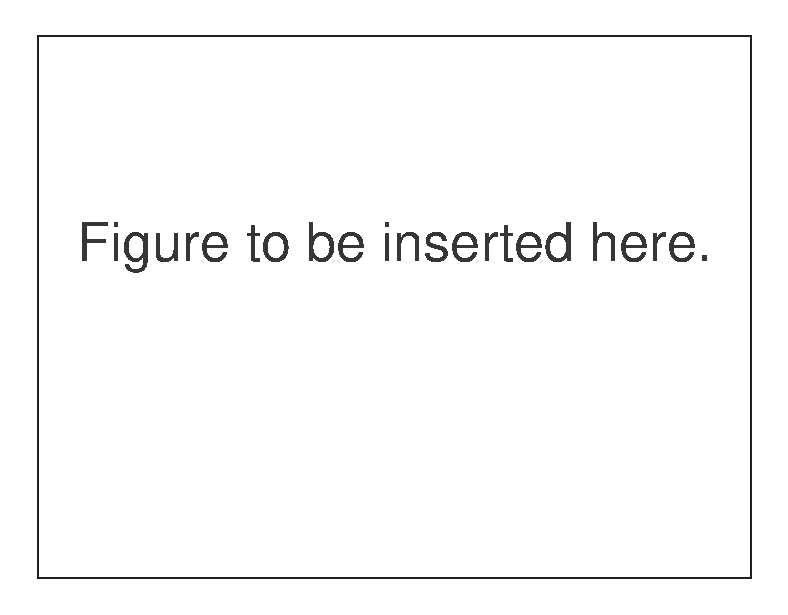
\includegraphics{./figures/BlankFigure.eps}}
\caption{Put caption here.}%
\label{fig:00}%
\end{center}
\end{figure}


\begin{figure}[t]
\begin{center}
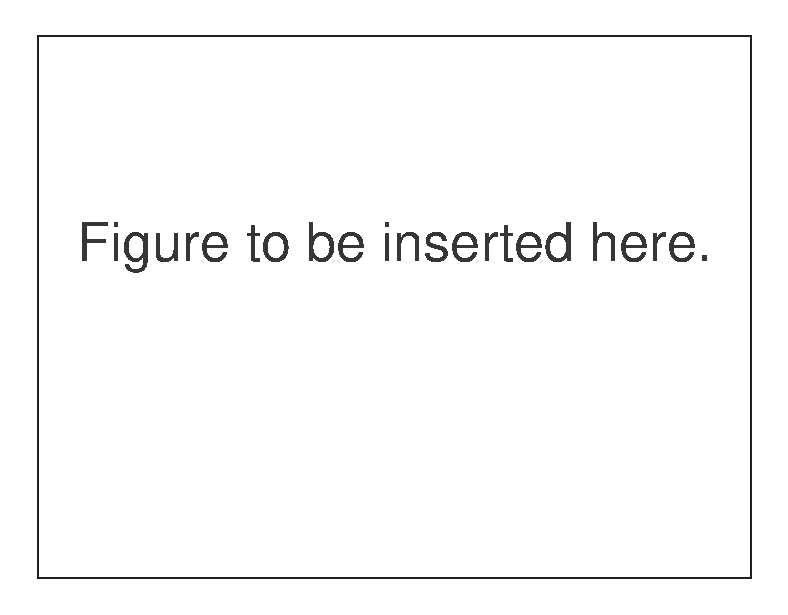
\includegraphics[width=12cm]{./figures/BlankFigure.eps}
\caption{Put caption here.}%
\label{fig:01}%
\end{center}
\end{figure}


\begin{figure}
\begin{center}
\begin{tabular}{cc}
\subfigure[aaa]{\epsfig{figure=./figures/BlankFigure.eps,width=5cm}}&
\subfigure[bbb]{\epsfig{figure=./figures/BlankFigure.eps,width=5cm}} \\
\end{tabular}
\end{center}
\caption{Put caption here.}
\label{fig:02}
\end{figure}

\bibliographystyle{plain}
\bibliography{myref}
\end{document}